\documentclass[12pt, oneside]{report}

\pdfcompresslevel=0
\pdfobjcompresslevel=\pdfcompresslevel

\usepackage[letterpaper, scale=0.92, centering]{geometry}
\usepackage{amssymb,amsmath,pifont,amsfonts,comment,enumerate}
\usepackage{currfile,xstring,hyperref,tabularx,graphicx,wasysym}
\usepackage{caption}
\usepackage[dvipsnames,table]{xcolor}
\usepackage{multicol,multirow,array,listings,tabularx,lastpage,textcomp,booktabs}

\usepackage{enumitem}
\usepackage{subcaption}
\usepackage{minted}
\usepackage{bookmark}

\setlength{\parindent}{0em}
\setlength{\parskip}{1em}

\hypersetup{
    colorlinks=true,
    linkcolor=black,%blue,
    filecolor=black,%magenta,      
    urlcolor=black,%cyan,
    pdftitle={Sharelatex Example},
    pdfpagemode=FullScreen
}

\captionsetup{hypcap=false}

\newcommand{\review}[0]{\textcolor{red}{REVIEW THIS}}
\newcommand{\chap}[1]{\chapter*{#1}\addcontentsline{toc}{chapter}{#1}}
\newcommand{\sect}[1]{\section*{#1}\addcontentsline{toc}{section}{#1}}
\newcommand{\subsect}[1]{\subsection*{#1}\addcontentsline{toc}{subsection}{#1}}
\newcommand{\subsubsect}[1]{\subsubsection*{#1}\addcontentsline{toc}{subsubsection}{#1}}

\usepackage{wrapfig}

\title{ECE 157C/272C HW 04\break{\Large A Complete Dataset Analytics Agent}}
\author{Caleb Harris}
\date{May 31$^\text{st}$, 2026}

\begin{document}
\setcounter{tocdepth}{2}

\graphicspath{ {./graphics} }

\begin{titlepage}
    \centering
    \pagenumbering{gobble}
    \maketitle
    \tableofcontents
    % \listoffigures
    % \listoftables
\end{titlepage}
\pagenumbering{arabic}

\clearpage
\graphicspath{ {./} }

%
%
\chap{Introduction}
%
%

\input{report-sections/01-introduction}

%
%
\chap{System Architecture}
%
%

\sect{Overview}

\begin{figure}[ht!]
  \centering
  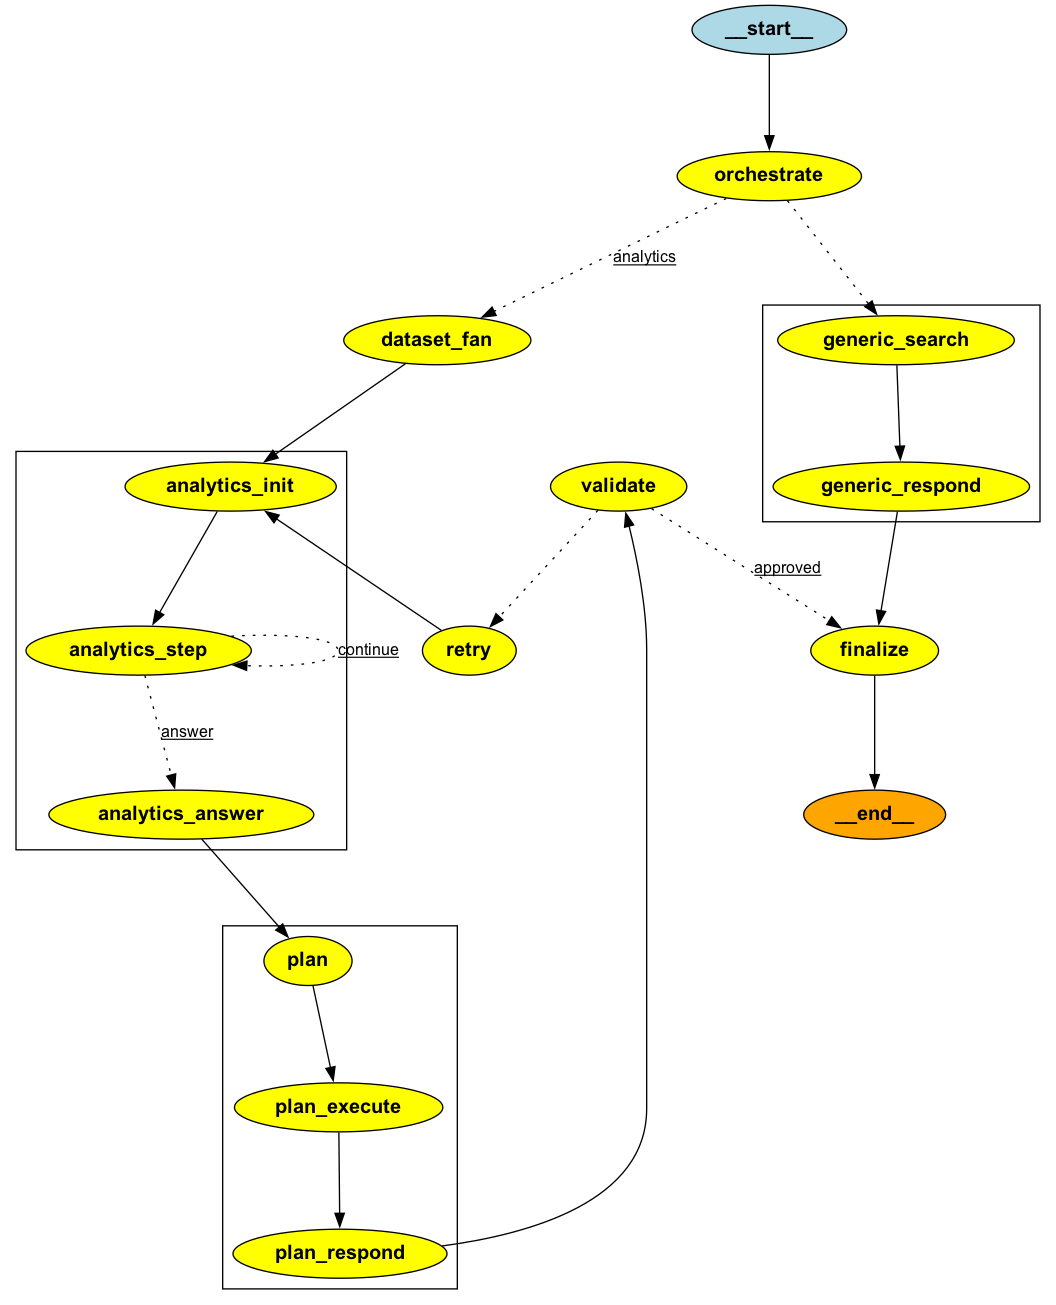
\includegraphics[width=0.4\textwidth]{graphics/graph-full.png}
  \caption{Full Agent Graph}
\end{figure}

The project implements a LangGraph-based analytics agent capable of answering
questions against CSV datasets, while also supporting a deterministic
plan-and-execute path and validation. The architecture combines:
\begin{itemize}
  \item An orchestration layer that routes questions to the appropriate path.
  \item A data-driven analytics subgraph that probes the datasets, iteratively
    analyzes data, and streams intermediate results (including plots).
  \item A deterministic plan-and-execute subgraph that translates a natural-language
    question into a sequence of data-transformations and then executes them.
  \item A validation subgraph that compares analytics results against the plan results
    to determine trustworthiness.
  \item A lightweight frontend/server that exposes the workflow and streams events to the user.
\end{itemize}

The following subsections summarize the core actors and their responsibilities.

\sect{Core Actors and Responsibilities}
\begin{itemize}
  \item \textbf{Orchestrator} (\texttt{orchestrator.py}):
    Decides whether a question should be handled via analytics with datasets or via a generic path.
    It converts the dataset question into a suitable prompt for downstream nodes and
    returns a decision along with an updated CSV path list for fan-out.

  \item \textbf{Dataset Fan-out} (\texttt{dataset\_node.py}):
    Profiles available datasets by reading CSV files from the datasets/ directory and
    constructing a schema that includes shapes and dtypes. It builds an initial execution
    namespace containing dataFrames for later analysis.

  \item \textbf{Analytics Agent} (\texttt{analytics\_agent.py}):
    Drives the data-driven exploration loop. It exposes three entry points:
    \subitem \texttt{analytics\_init\_node}: initializes thought space and the first step.
    \subitem \texttt{analytics\_step\_node}: performs iterative analysis by asking the LLM for
    reasoning; may generate executable Python code to run against the namespace.
    \subitem \texttt{analytics\_answer\_node}: aggregates the final analytics answer, plots, and step history.
    The analytics loop streams plots and answers as the analysis progresses.

  \item \textbf{Plan-and-Execute Subgraph} (\texttt{plan\_planner.py}, \texttt{plan\_executor.py}, \texttt{plan\_operators.py}, \texttt{plan\_schemas.py}, \texttt{plan\_respond.py}):
    A deterministic planning module.
    \subitem The planner translates a natural-language question into a strict JSON plan (op sequence)
    that operates on the dataset (load\_dataset is always the first step).
    \subitem The executor applies the plan to the active DataFrame, recording a trace of
    inputs/outputs and collecting an execution result.
    \subitem The responder converts the execution outcome into a final answer, using LLM-driven
    reasoning to describe the plan-derived results.

  \item \textbf{Validator} (\texttt{validator.py}):
    Independently assesses the analytics and plan outputs for consistency. It returns a verdict
    (pass/retry/flag) along with a rationale and optional missing items. Retries are handled by a
    separate retry node that preserves baseline state.

  \item \textbf{Finalization and Frontend} (\texttt{finalize.py}, \texttt{server.py}, frontend.html):
    The backend server streams events to the frontend via Server-Sent Events (SSE). The frontend
    presents a live feed of the analysis, including per-step reasoning, code, plots, and the final
    answer.
\end{itemize}

\sect{Data Flow and State Model}
The runtime state is modeled as a structured JSON-like object (GraphState) defined in
\textbf{\texttt{schemas.py}}. Key facets include:
\begin{itemize}
  \item \emph{Inputs}: \{ question, csv\_paths \} describing the user query and the
    datasets to consider.
  \item \emph{Orchestration}: a decision payload (orchestration\_decision) and initial dataset
    thoughts (dataset\_thoughts).
  \item \emph{Analytics State}: an execution namespace (namespace), a sequence of analytic steps
    (steps), collected plots (plots), the index of the current step (current\_step\_index), and a flag
    is\_complete.
  \item \emph{Plan-Execute State}: a concrete plan (plan), a trace of executed steps (trace),
    the textual execution output (execution\_result), and the final answer (final\_answer).
  \item \emph{Validation and Results}: a validation\_result, retry counters and feedback, and
    any final plots or answers.
\end{itemize}

\sect{Interaction Model and Interfaces}
The components communicate primarily through strongly-typed Python data models (Pydantic)
defined in \texttt{\texttt{schemas.py}} and JSON payloads produced/consumed by the LLM utilities
in \texttt{utilities/}. Key interaction patterns include:
\begin{itemize}
  \item LLM routing: the orchestrator calls an LLM (via \texttt{call\_llm}) to obtain an
    orchestration decision, which directs the subsequent path.
  \item Analytics loop: the analytics node uses an iterative prompt/response pattern to refine
    the analysis steps, producing executable code when needed, and streaming plots via the
    namespace for downstream collection.
  \item Deterministic planning: the planner uses a strict DSL of data-transform operations to
    ensure reproducibility, with a first required step of \texttt{load\_dataset}.
  \item Validation and retries: the validator provides a verdict that can trigger a retry with
    retained baseline state to ensure robustness.
\end{itemize}

\sect{Notes and Extensibility}

The architecture emphasizes modularity: swapping a node or extending the DSL requires minimal changes to the graph wiring and configuration prompts.

The system is designed to stream results progressively (steps, plots, final answer) to support interactive use in the provided frontend.


%
%
\chap{Component Design}
%
%

%
\sect{Orchestrator}
%

The Orchestrator is the entry point in the data-question graph. It decides whether a given user question should be answered via the analytics/data-driven path or via a generic knowledge path, and it prepares the inputs for the downstream subgraphs.

\begin{itemize}
  \item \textbf{Python mapping}: \texttt{orchestrator.py}
  \item \textbf{Key schemas}: GraphState, \texttt{OrchestrationDecision} (from \texttt{schemas.py})
  \item \textbf{Role}: Route questions to the appropriate path, and prepare the initial CSV path list for fan-out.
  \item \textbf{How it operates}:
    \subitem Builds a minimal prompt from the incoming state:
    \texttt{Question:} {state["question"]}
    \subitem Calls the LLM with a response model of \texttt{\texttt{OrchestrationDecision}}. The LLM returns a structured decision indicating either the analytics path or the generic path, together with a brief justification.
    \subitem Returns a dictionary containing:
    \texttt{\{"csv\_paths": [...], "orchestration\_decision": orchestration\_decision, "retry\_count": 0\}}
  \item \textbf{Inputs}:
      \subitem \texttt{state["question"]}: the user query text
      \subitem \texttt{state["csv\_paths"]}: list of CSV dataset paths to be considered downstream
    \item \textbf{Outputs}:
      \subitem \texttt{\{"csv\_paths": [...], \"orchestration\_decision\": decision, \"retry\_count\": 0\}}
  \item \textbf{Prompts design / structure}:
      \subitem System prompt: empty (delegates the routing decision to the LLM)
      \subitem User prompt: a concise Question block:
        \texttt{Question:} {state["question"]}
      \subitem The LLM is expected to return a calibrated \texttt{OrchestrationDecision} object with fields such as:
        \texttt{agent\_type}: \texttt{"analytics"} or \texttt{"generic"}
        \texttt{reasoning}: a short justification for the routing decision
      \subitem The implementation uses the \texttt{OrchestrationDecision} model to validate and parse the response.
\end{itemize}


%
\sect{Analytics Agent}
%

\subsect{Dataset Understanding Node (dataset\_node.py)}
The Dataset Understanding node performs the fan-out preparation by inspecting the provided CSV datasets, extracting basic schema information, and exposing a namespace for downstream analytics.

\begin{itemize}
  \item \textbf{Python mapping}: dataset\_node.py
  \item \textbf{Key schemas}: DatasetThoughts (from schemas.py), PLOTLY\_NAMESPACE\_KEY (from schemas.py), GraphState
  \item \textbf{Role}: Profile available datasets, build initial dataset schemas (shape and dtypes), and construct a sandbox namespace for analytics code execution.
  \item \textbf{How it operates}:
    \subitem Iterates over state["csv\_paths"], loads each CSV from the datasets/ directory into a pandas DataFrame, and records its shape and column types.
    \subitem Constructs a per-dataset schema dictionary and a namespace containing dataFrames and a dedicated Plotly namespace for capturing plots.
    \subitem Calls the LLM with a system prompt that instructs returning ONLY a JSON object with {
    (note: two fields) reasoning and schemas } where:
    \subitem reasoning: rationale for column selection and dataset approach
    \subitem schemas: the dataset schemas to guide downstream processing
    \subitem Validates the LLM response into a DatasetThoughts model.
  \item \textbf{Inputs}: state["question"], state["csv\_paths"]
  \item \textbf{Outputs}: {"dataset\_thoughts": DatasetThoughts, "namespace": {PLOTLY\_NAMESPACE\_KEY: {}, "dataFrames": dataFrames}}
  \item \textbf{Prompts design / structure}:
    \subitem System prompt explicitly requests a JSON with two fields: reasoning and schemas.
    \subitem User prompt includes the Question and Unfiltered Dataset Specifications serialized as JSON.
    \subitem The LLM return is parsed into the DatasetThoughts model so downstream components can rely on a typed structure.
\end{itemize}

\subsect{Analytics Agent Node (analytics\_agent.py)}
The Analytics Agent node implements the data-driven exploration loop that iteratively reasons about the dataset and (optionally) generates executable Python to compute the answer.

\begin{itemize}
  \item \textbf{Python mapping}: analytics\_agent.py
  \item \textbf{Key schemas}: Plot, GraphState, AnalyticsStep, AnalyticsReasoning, AnalyticsAction, AnalyticsFinalAnswer, AnalyticsResult, PLOTLY\_NAMESPACE\_KEY
  \item \textbf{Role}: Drive the data-driven exploration loop, including: init step, iterative reasoning/code generation steps, and final answer synthesis.
  \item \textbf{How it operates}:
    \subitem analytics\_init\_node: runs a tiny Python snippet in the sandbox to reveal dataFrames keys; appends dataset schemas to stdout; returns initial AnalyticsStep with reasoning and code.
    \subitem analytics\_step\_node: constructs a prompt from the question, prior steps, and any retry feedback; asks the LLM for AnalyticsReasoning. If the model indicates Python execution is required, it asks for AnalyticsAction (code), executes it in the sandbox, harvests any plots, and appends a new AnalyticsStep with code and execution results.
    \subitem analytics\_answer\_node: prompts for final AnalyticsFinalAnswer after the last step; compiles an AnalyticsResult with final\_answer, overall\_plan, and the collected steps/plots.
  \item \textbf{Inputs}: state including question, namespace, steps, plots, retry\_count, dataset\_thoughts, etc.
  \item \textbf{Outputs}: {"analytics\_result": AnalyticsResult}
  \item \textbf{Prompts design / structure}:
    \subitem Three LLM prompts:
  1) AnalyticsReasoning: outputs AnalyticsReasoning with reasoning and a flag requires\_python\_execution.
  2) AnalyticsAction: outputs code to execute in the sandbox; code follows sandbox conventions (imports at top, print calls, and Plotly capture via \_plotly).
  3) AnalyticsFinalAnswer: outputs final answer and overall plan.
  \item \textbf{Sandbox conventions}:
  \subitem namespace persists across steps; use print() for outputs; capture plots via: \_plotly["Title"] = fig.to\_json(); do not call fig.show().
\end{itemize}


%
\sect{Plan and Execute Agent}
%

The Plan and Execute Agent provides a deterministic, reproducible pipeline for answering questions via a strict plan of data-transform operations.

\begin{center}
  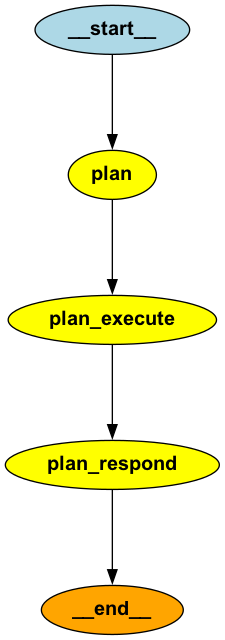
\includegraphics[width=0.13\textwidth]{graphics/graph-plan_and_execute.png}
  \captionof{figure}{Plan and Execute Agent Graph}
\end{center}

\begin{itemize}
  \item \textbf{Python mappings}: plan\_planner.py, plan\_executor.py, plan\_respond.py
  \item \textbf{Key schemas}: PlanToExecute, PlanExecuteFinalAnswer, Step types (from plan\_schemas.py), TraceEntry, DatasetEntry
  \item \textbf{Role}: Produce a deterministic plan (via plan\_planner), execute it (plan\_executor) against the dataset, and synthesize a final natural-language answer (plan\_respond).
  \item \textbf{How it operates}:
    \subitem Plan node (plan\_planner.py): receives the question and dataset paths; calls the LLM with PLANNER\_SYSTEM\_PROMPT to produce a strict JSON PlanToExecute, validating with PlanToExecute.model\_validate\_json. Returns plan\_execute\_result with plan and empty trace/execution\_result/final\_answer.
    \subitem Plan executor (plan\_executor.py): walks the plan's steps, applying each operation to the active DataFrame using plan\_operators.dispatch\_op, recording a trace of inputs/outputs and any errors. Supports snapshot/restore, joins, and concatenations via the DSL.
    \subitem Plan respond (plan\_respond.py): converts the final execution outcome into a PlanExecuteFinalAnswer using a dedicated LLM prompt that summarizes the execution and results.
  \item \textbf{Inputs}: state including question, csv\_paths, and dataset context; the planner's output is consumed by the executor.
  \item \textbf{Outputs}: PlanToExecute (from plan\_node), plan\_execute\_result (with final\_answer and trace), PlanExecuteFinalAnswer (for final natural-language answer).
  \item \textbf{Prompts design / structure}:
    \subitem The planner uses a DSL of operations: load\_dataset, select\_columns, rename\_columns, filter\_rows, derive\_columns, reduce\_columns, normalize\_columns, rank, group\_aggregate, sort\_rows, limit\_rows, distinct\_rows, pivot, snapshot, restore, join, concat, display.
    \subitem The plan\_node enforces the first step to be load\_dataset and uses a JSON structure for steps.
    \subitem plan\_executor uses plan\_operators to apply each Step to a DataFrame and records a trace for each step.
\end{itemize}


%
\sect{Validator Agent}
%

The Validator node provides a safety check by comparing the analytics output with the plan-execute results and deciding whether to finalize or retry.

\begin{itemize}
  \item \textbf{Python mapping}: validator.py
  \item \textbf{Key schemas}: ValidationDecision (from schemas.py)
  \item \textbf{Role}: Validate results, trigger retries if needed, and preserve baseline state for stable retries.
  \item \textbf{How it operates}:
    \subitem validation\_node(state, config): Deep copies analytics\_result and plan\_execute\_result; strips nonessential fields; prompts the LLM with a concise comparison between Analytics final\_answer and Plan final\_answer, requesting a ValidationDecision.
    \subitem retry\_node(state, config): When verdict is retry, increments retry\_count, preserves plan\_execute\_result, clears analytics\_result for re-run, and resets navigation state for a fresh analytics loop.
  \item \textbf{Inputs}: state including question, analytics\_result, plan\_execute\_result, retry\_count, validation\_result.
  \item \textbf{Outputs}: {"validation\_result": ValidationDecision} or a next-state dict in case of retry.
  \item \textbf{Prompts design / structure}:
    \subitem The prompt is a compact synthesis of the analytics vs plan results to drive the LLM verdict.
\end{itemize}


%
%
\chap{Dataset Exploration}
%
%

\begin{center}
  \hyperlink{https://www.kaggle.com/datasets/cnic92/200-financial-indicators-of-us-stocks-20142018}{\textit{200+ Financial Indicators of US stocks (2014-2018)}}
\end{center}

The dataset consists of five annual CSV files spanning 2014 through 2018, each containing approximately 4000 rows and 223 financial indicator columns. Rows correspond to individual company-year observations identified by a ticker symbol and a sector label. The dataset was assembled from the Financial Modeling Prep API and pandas-datareader and is available on Kaggle under the title 200+ Financial Indicators of US Stocks (2014-2018).

Across the five files, 4980 distinct ticker symbols appear, though not every ticker is present in every year — the year-over-year overlap is roughly $74.82\%$, reflecting delistings, IPOs, and coverage gaps in the source API. Financial Services is the most heavily represented sector in every year, accounting for approximately $21.38\%$ of unique tickers annually, followed by Healthcare and Technology. The remaining sectors — Industrials, Consumer Cyclical, Basic Materials, Real Estate, Utilities, Energy, Consumer Defensive, and Communication Services — each contribute a smaller and comparatively stable share.

Missing values are pervasive. There are roughly 5 million cells; $16.61\%$ are \texttt{NaN}. Columns representing less common indicators (e.g., net debt to EBITDA, free cash flow yield) have substantially higher \texttt{NaN} rates than core metrics like revenue or EPS. The author of the dataset notes the presence of outliers likely caused by data-entry errors; inspection confirms that several indicators contain values orders of magnitude larger than the interquartile range, which motivated the winsorization step often used in the analytics agent's preprocessing pipeline.

These characteristics shaped several architectural decisions. The \texttt{NaN} density made it impractical to require all 223 columns to be populated for a row to be valid; instead, the analytics agent selects and cleans only the columns relevant to each query. The outlier distribution motivated the use of median rather than mean aggregation in sector-level comparisons, and explicit winsorization before z-score normalization in composite scoring tasks.


%
%
\chap{Representative Examples}
%
%

%
\sect{Generic Question 1}
%

\begin{wrapfigure}{l}{0pt}
  \centering
  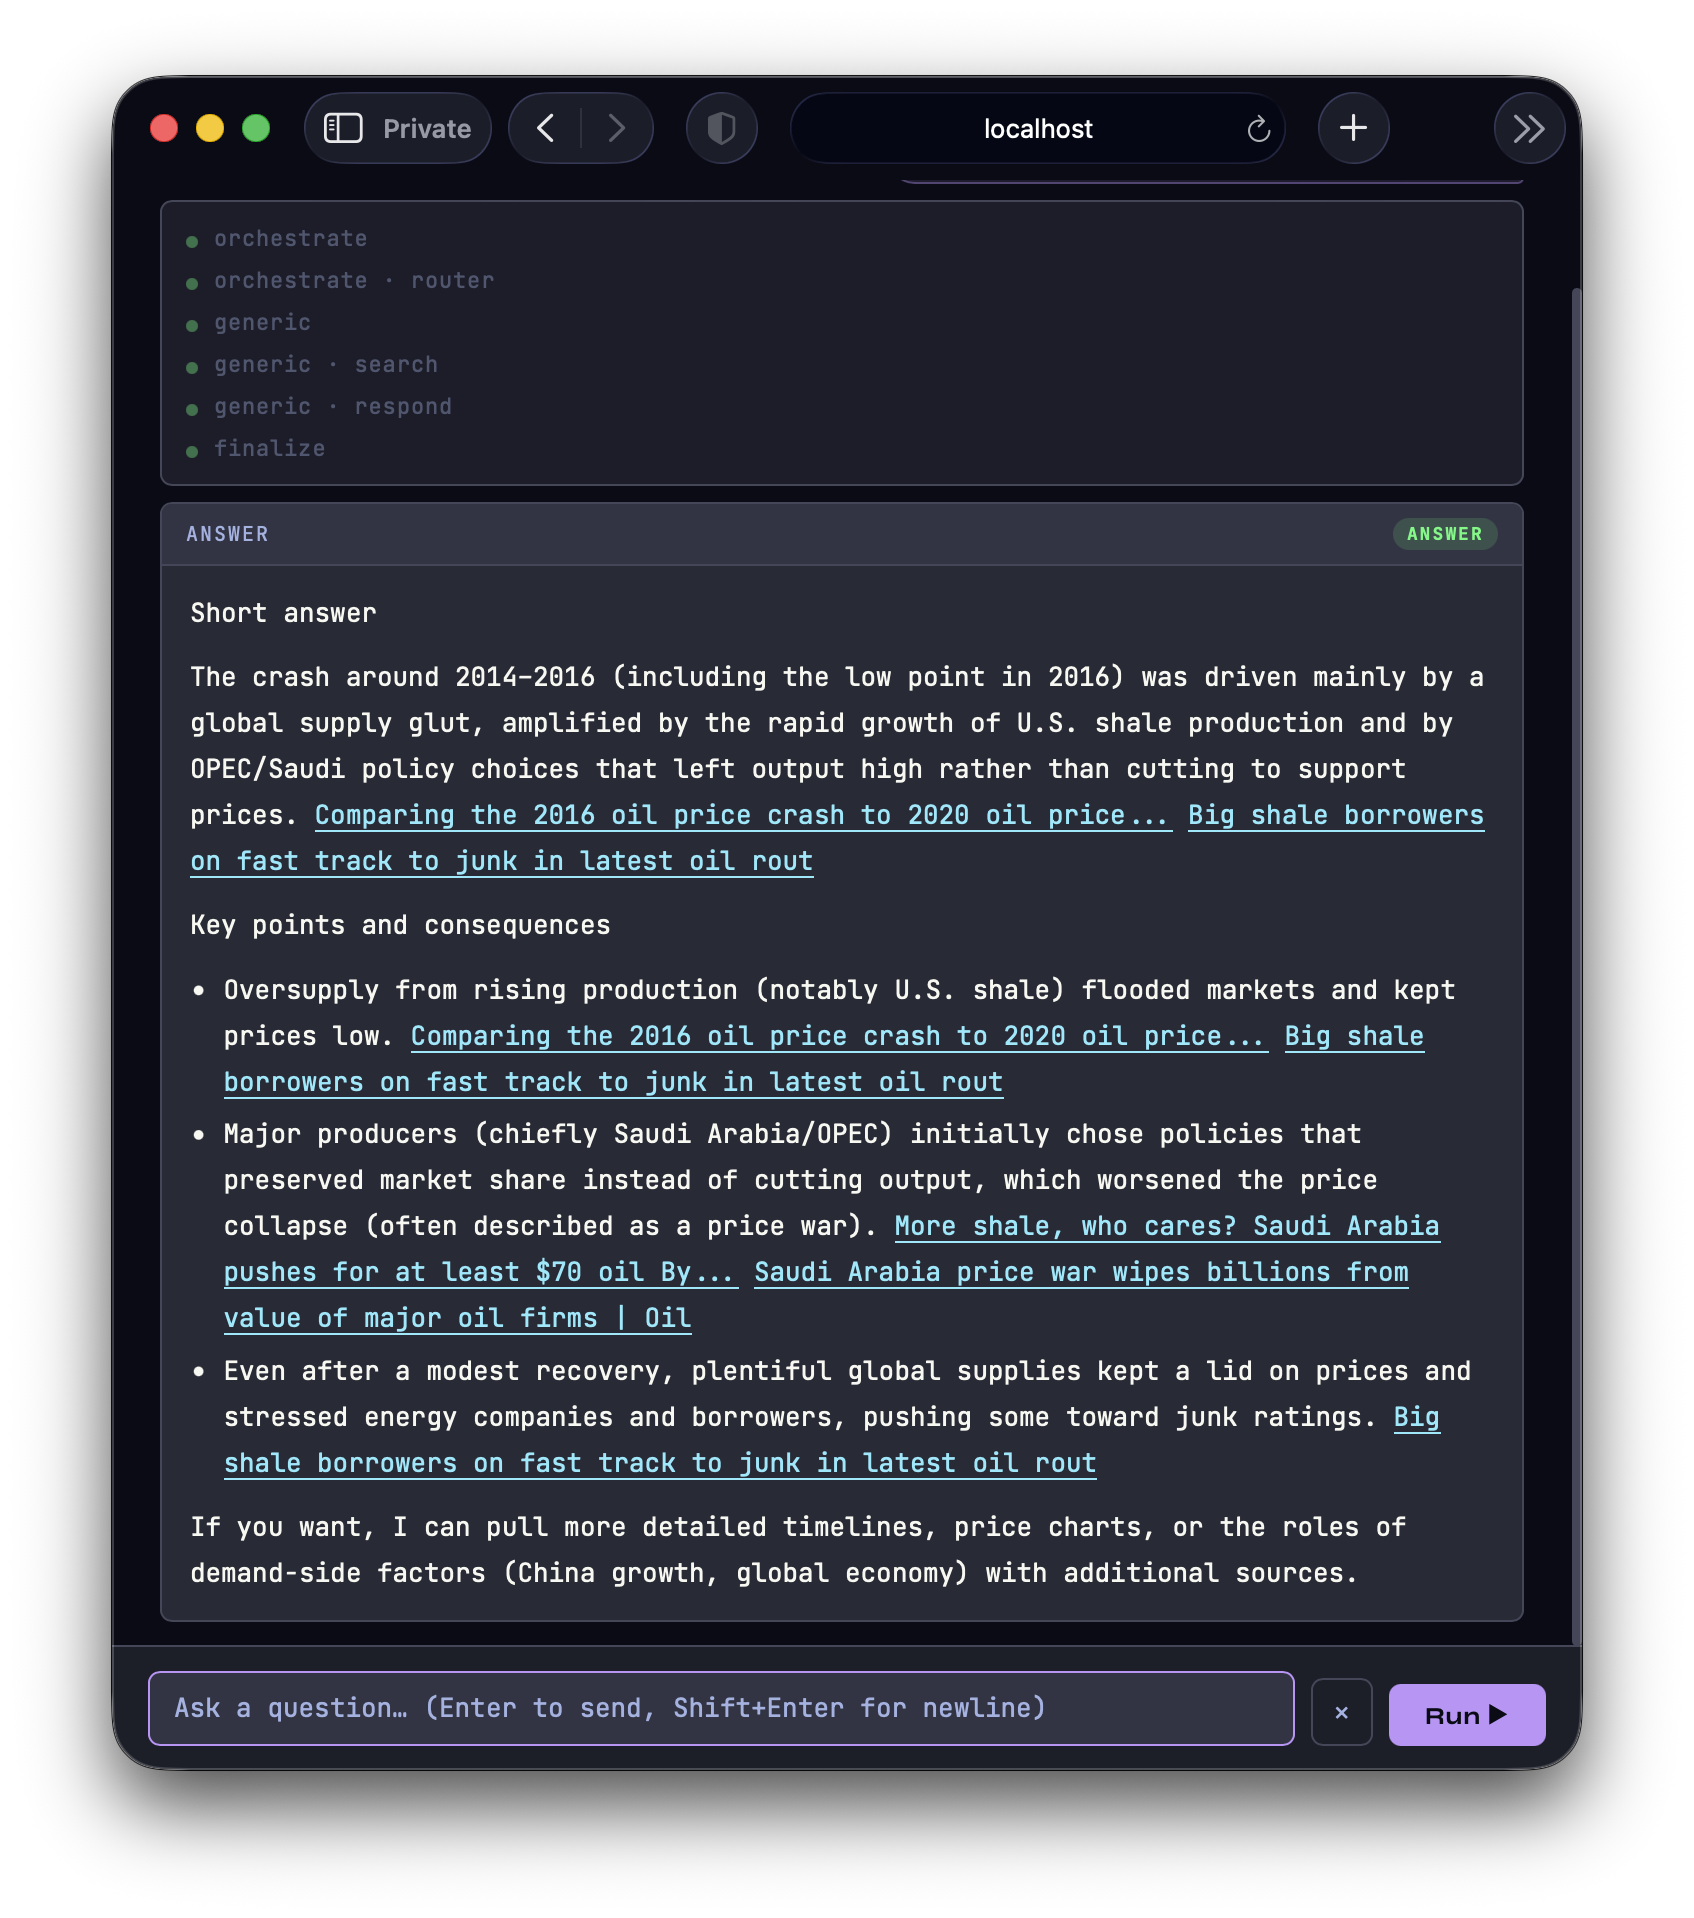
\includegraphics[width=0.4\textwidth]{graphics/ui-what-caused-the-2016-oil-price-crash.png}
  \caption{UI Screenshot}
\end{wrapfigure}

The primary goal was to identify and explain the confluence of factors responsible for the sharp decline in global oil prices around 2016. The agent utilized a multi-step process involving information retrieval, causal relationship mapping, and synthesis across various economic reports.

\subsect{Step 1: Information Retrieval \& Scope Definition}
The query was broken down into key search concepts: (a) timeline/event ("2016 oil price crash"), (b) mechanisms of collapse (causes), and (c) major industry players (OPEC, Saudi Arabia, U.S. Shale). The agent successfully retrieved several articles establishing the context:
\begin{itemize}
  \item \textbf{Timeline Confirmation:} Sources confirmed that the collapse was a protracted event spanning 2014–2016 [Nairametrics].
  \item \textbf{Key Players/Factors:} Results highlighted the roles of U.S. shale oversupply, OPEC decisions, and Saudi policy (price war).
\end{itemize}

\subsect{Step 2: Causal Factor Analysis \& Mapping}
The agent did not simply list facts; it analyzed *how* these factors interacted to create a collapse. Two primary causal dimensions were mapped:

\subsubsect{A) Supply-Side Pressure (Oversupply)}
Multiple sources pointed to an unchecked increase in global supply as the fundamental trigger. The rapid development and output of U.S. shale production played a critical role, overwhelming market capacity and keeping prices suppressed [Nairametrics]. This established the base condition: persistent oversupply.

\subsubsect{B) Policy Failure (Producer Behavior)}
The agent identified that the response from major producers was exacerbating, rather than mitigating, the crisis. Key findings showed:
\begin{itemize}
\item Saudi Arabia's attempts to maintain market value by refusing deep cuts [Investing].
\item The resulting "price war" among major firms, which wiped out billions in market value [The Guardian].
\end{itemize}
This established that the policy decision (maintaining output share vs. cutting supply) actively worsened the price decline.

\subsect{Step 3: Synthesis and Structuring the Answer}
Finally, the agent synthesized these two dimensions into a cohesive narrative structure suitable for a report summary, defining the collapse as the interaction of market oversupply $\textbf{plus}$ poor policy coordination. The final answer clearly delineates the key points:

\begin{enumerate}
\item \textbf{Root Cause:} Global supply glut (Shale).
\item \textbf{Amplifying Factor:} Producer decisions that prevented necessary output cuts (Policy/Price War).
\item \textbf{Consequence:} Prices remained capped despite recovery attempts, posing financial risks to energy sectors and borrowers.
\end{enumerate}

This systematic approach ensured the answer was not merely a collection of facts but a detailed explanation of the complex economic mechanism that led to the 2016 oil price crash.


\break

%
\sect{Generic Question 2}
%

\begin{wrapfigure}{l}{0pt}
  \centering
  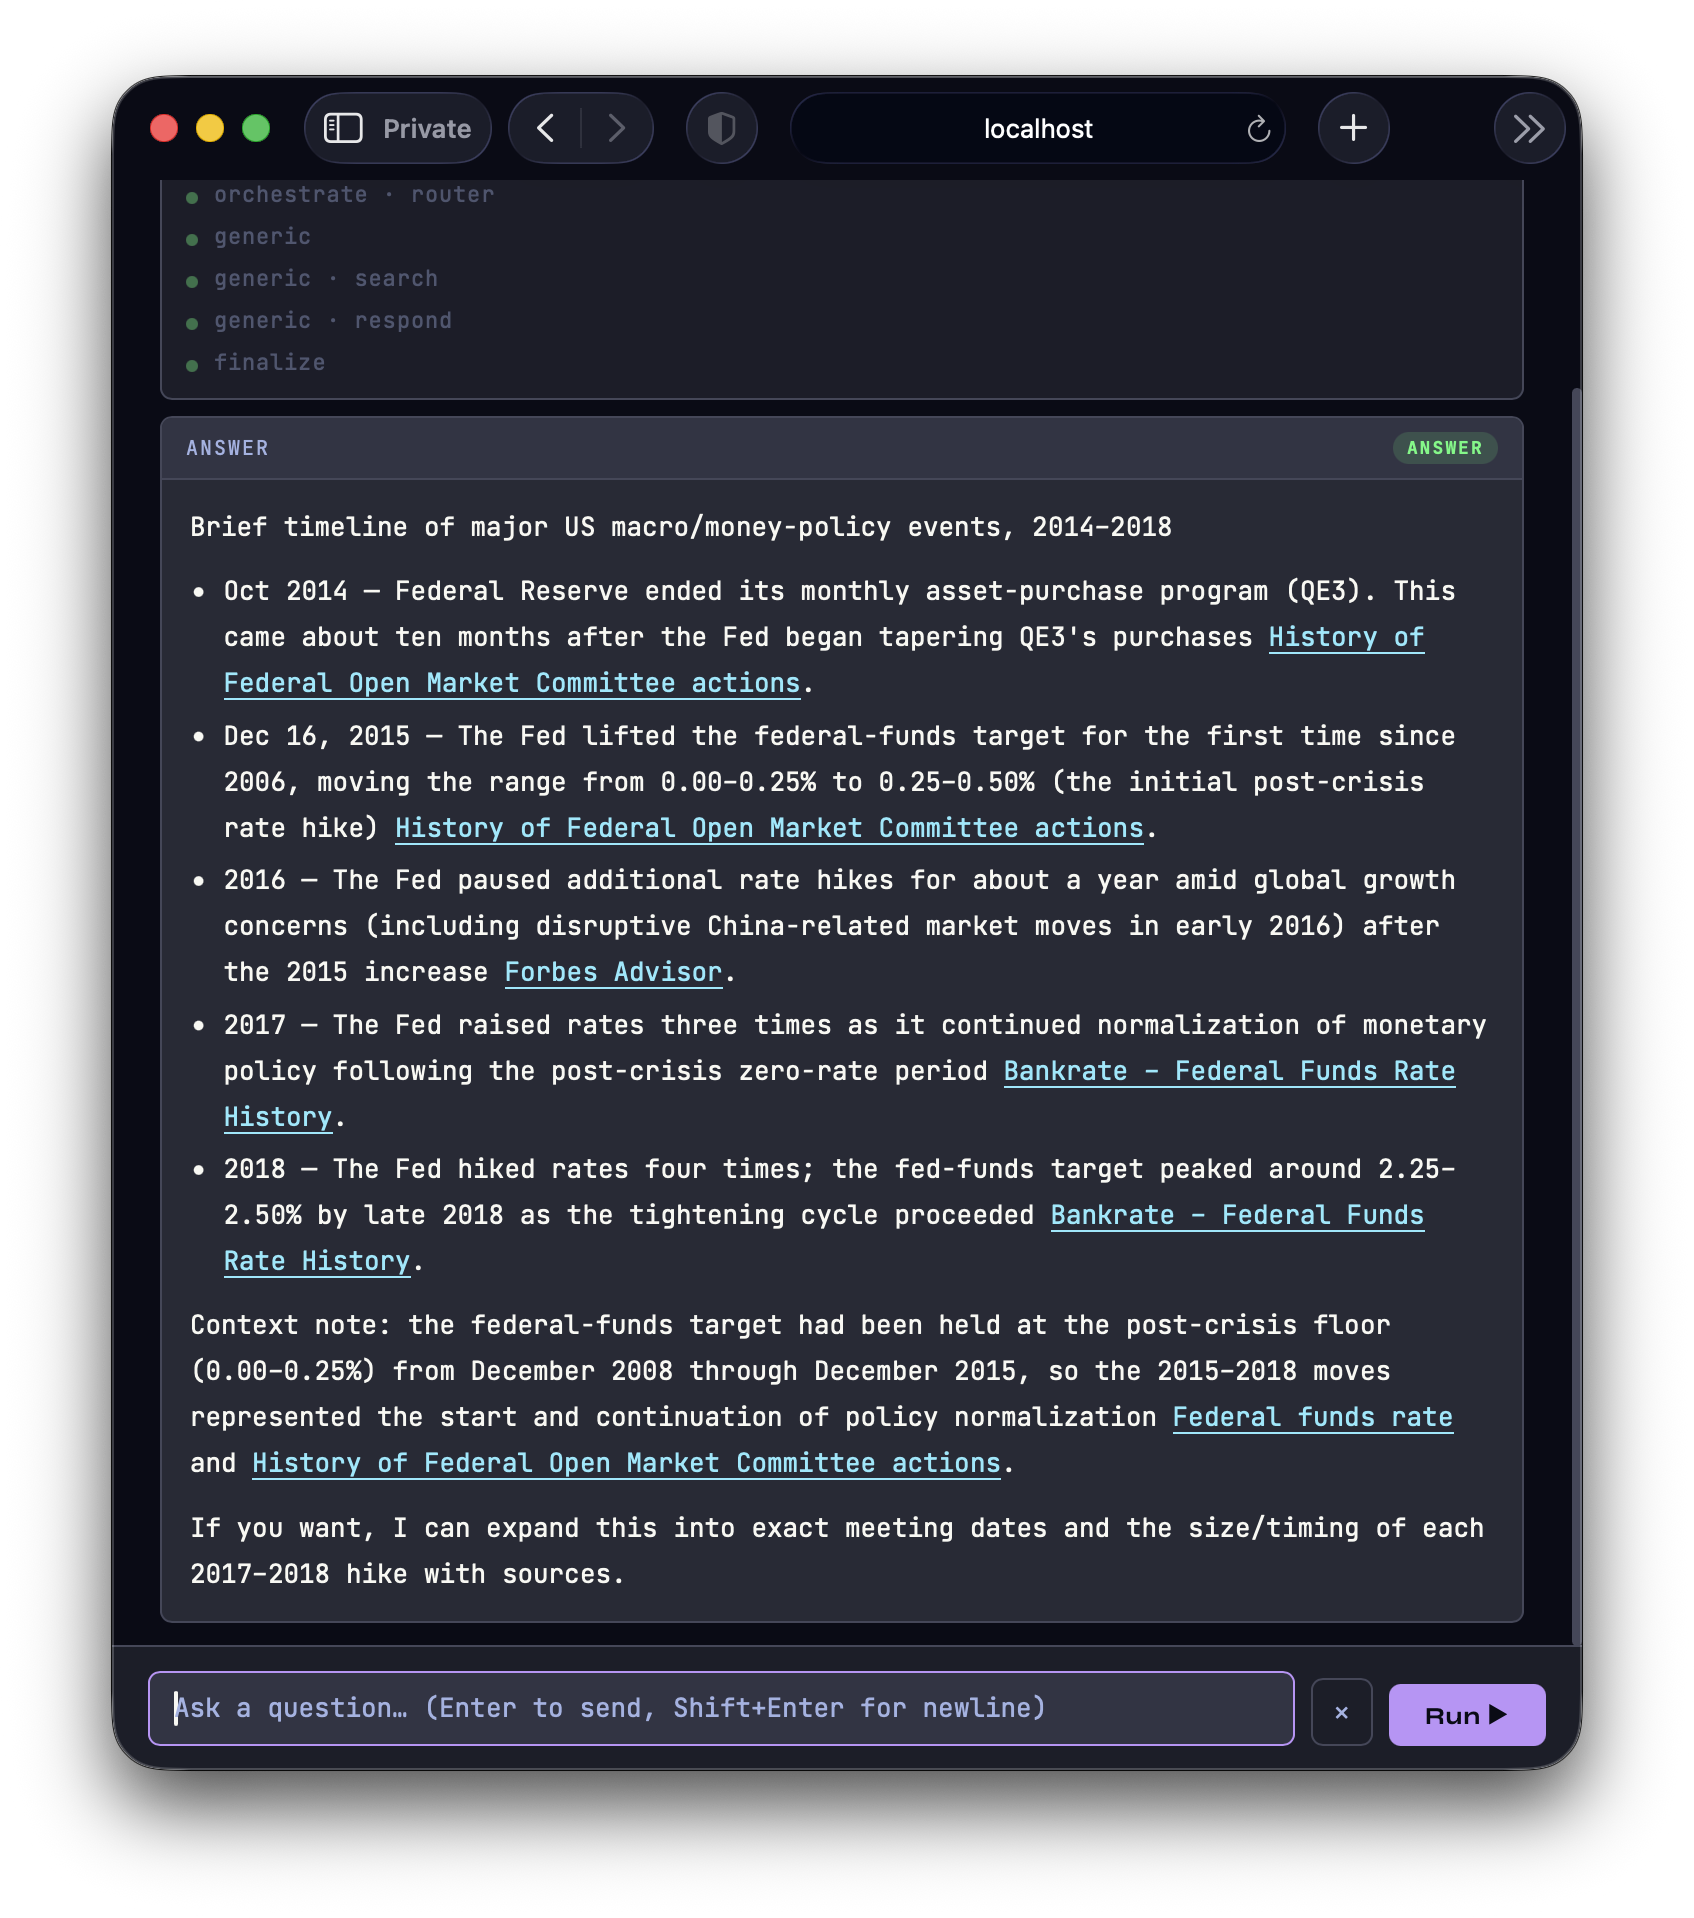
\includegraphics[width=0.4\textwidth]{graphics/ui-what-us-macroeconomic-events-rate-hikes,-policy-changes-occurred-between-2014-and-2018.png}
  \caption{UI Screenshot}
\end{wrapfigure}

The objective was to construct a chronological timeline of major US monetary policy shifts, specifically focusing on Federal Reserve actions (rate hikes and quantitative easing changes) between 2014 and 2018. The agent employed a temporal analysis strategy, prioritizing date keywords (\textit{2014}, \textit{2015}, \textit{2016}, \textit{2017}, \textit{2018}) and policy-specific terms (\textit{QE}, \textit{rate hike}, \textit{Federal Funds Rate}, \textit{tapering}).

\subsect{Step 1: Establishing the Starting Point (2014)}
The agent first queried for major shifts near the start date. The search results immediately highlighted the end of Quantitative Easing (QE3). Source [Wikipedia - OMF Committee actions] confirmed that the Federal Reserve ended its monthly asset purchases program (QE3) in \textbf{October 2014}, noting this followed a tapering process, thus marking a major policy shift from accommodative monetary policy.

\subsect{Step 2: Identifying the First Rate Hike (2015)}
The agent then focused on rate normalization post-crisis. Source [Wikipedia - OMF Committee actions] and [Forbes Advisor] consistently identified the critical event of \textbf{December 16, 2015}. The key action was raising the Federal Funds Rate for the first time since 2006, moving the target range from $0.00-0.25\%$ to $0.25-0.50\%$. This step established the start of "policy normalization."

\subsect{Step 3: Tracking Cyclical Changes and Pauses (2016-2018)}
The agent analyzed rate movements year-by-year.
\begin{itemize}
  \item \textbf{2016:} Source [Forbes Advisor] introduced the concept of a pause. The agent extracted that following the 2015 hike, the Fed paused additional rate hikes for approximately a year due to global growth concerns, specifically mentioning disruptive China-related market moves in early 2016.
  \item \textbf{2017:} Source [Bankrate] and [final\_answer.md] provided specific quantification. The agent determined that the Fed resumed hiking rates three times during 2017 as part of continued normalization efforts.
  \item \textbf{2018:} The trend accelerated. Source [Bankrate] confirmed that rates were raised four times in 2018, leading to a peak target rate near $2.25\%–2.50\%$ by the end of the year. This completed the tightening cycle phase analyzed.
\end{itemize}

\subsect{Step 4: Synthesis and Timeline Construction}
Finally, the agent synthesized these discrete points into a coherent narrative timeline, ensuring that the overall context (the shift from a multi-year zero-rate environment to aggressive normalization) was maintained. The agent used the contextual notes provided in $\text{\texttt{final\_answer.md}}$ to frame the entire period as "the start and continuation of policy normalization," providing a high-level summary ideal for the final answer structure.

\subsect{Conclusion}
The process successfully gathered both the specific dates/amounts (e.g., Dec 2015 rate hike) and the overarching narrative context (policy tightening cycle $2017 \rightarrow 2018$; pause in $2016$), resulting in a comprehensive, chronological report of major US macroeconomic policy shifts during the target window.


\break

%
\sect{Analytics Question 1}
%

\begin{wrapfigure}{l}{0pt}
  \centering
  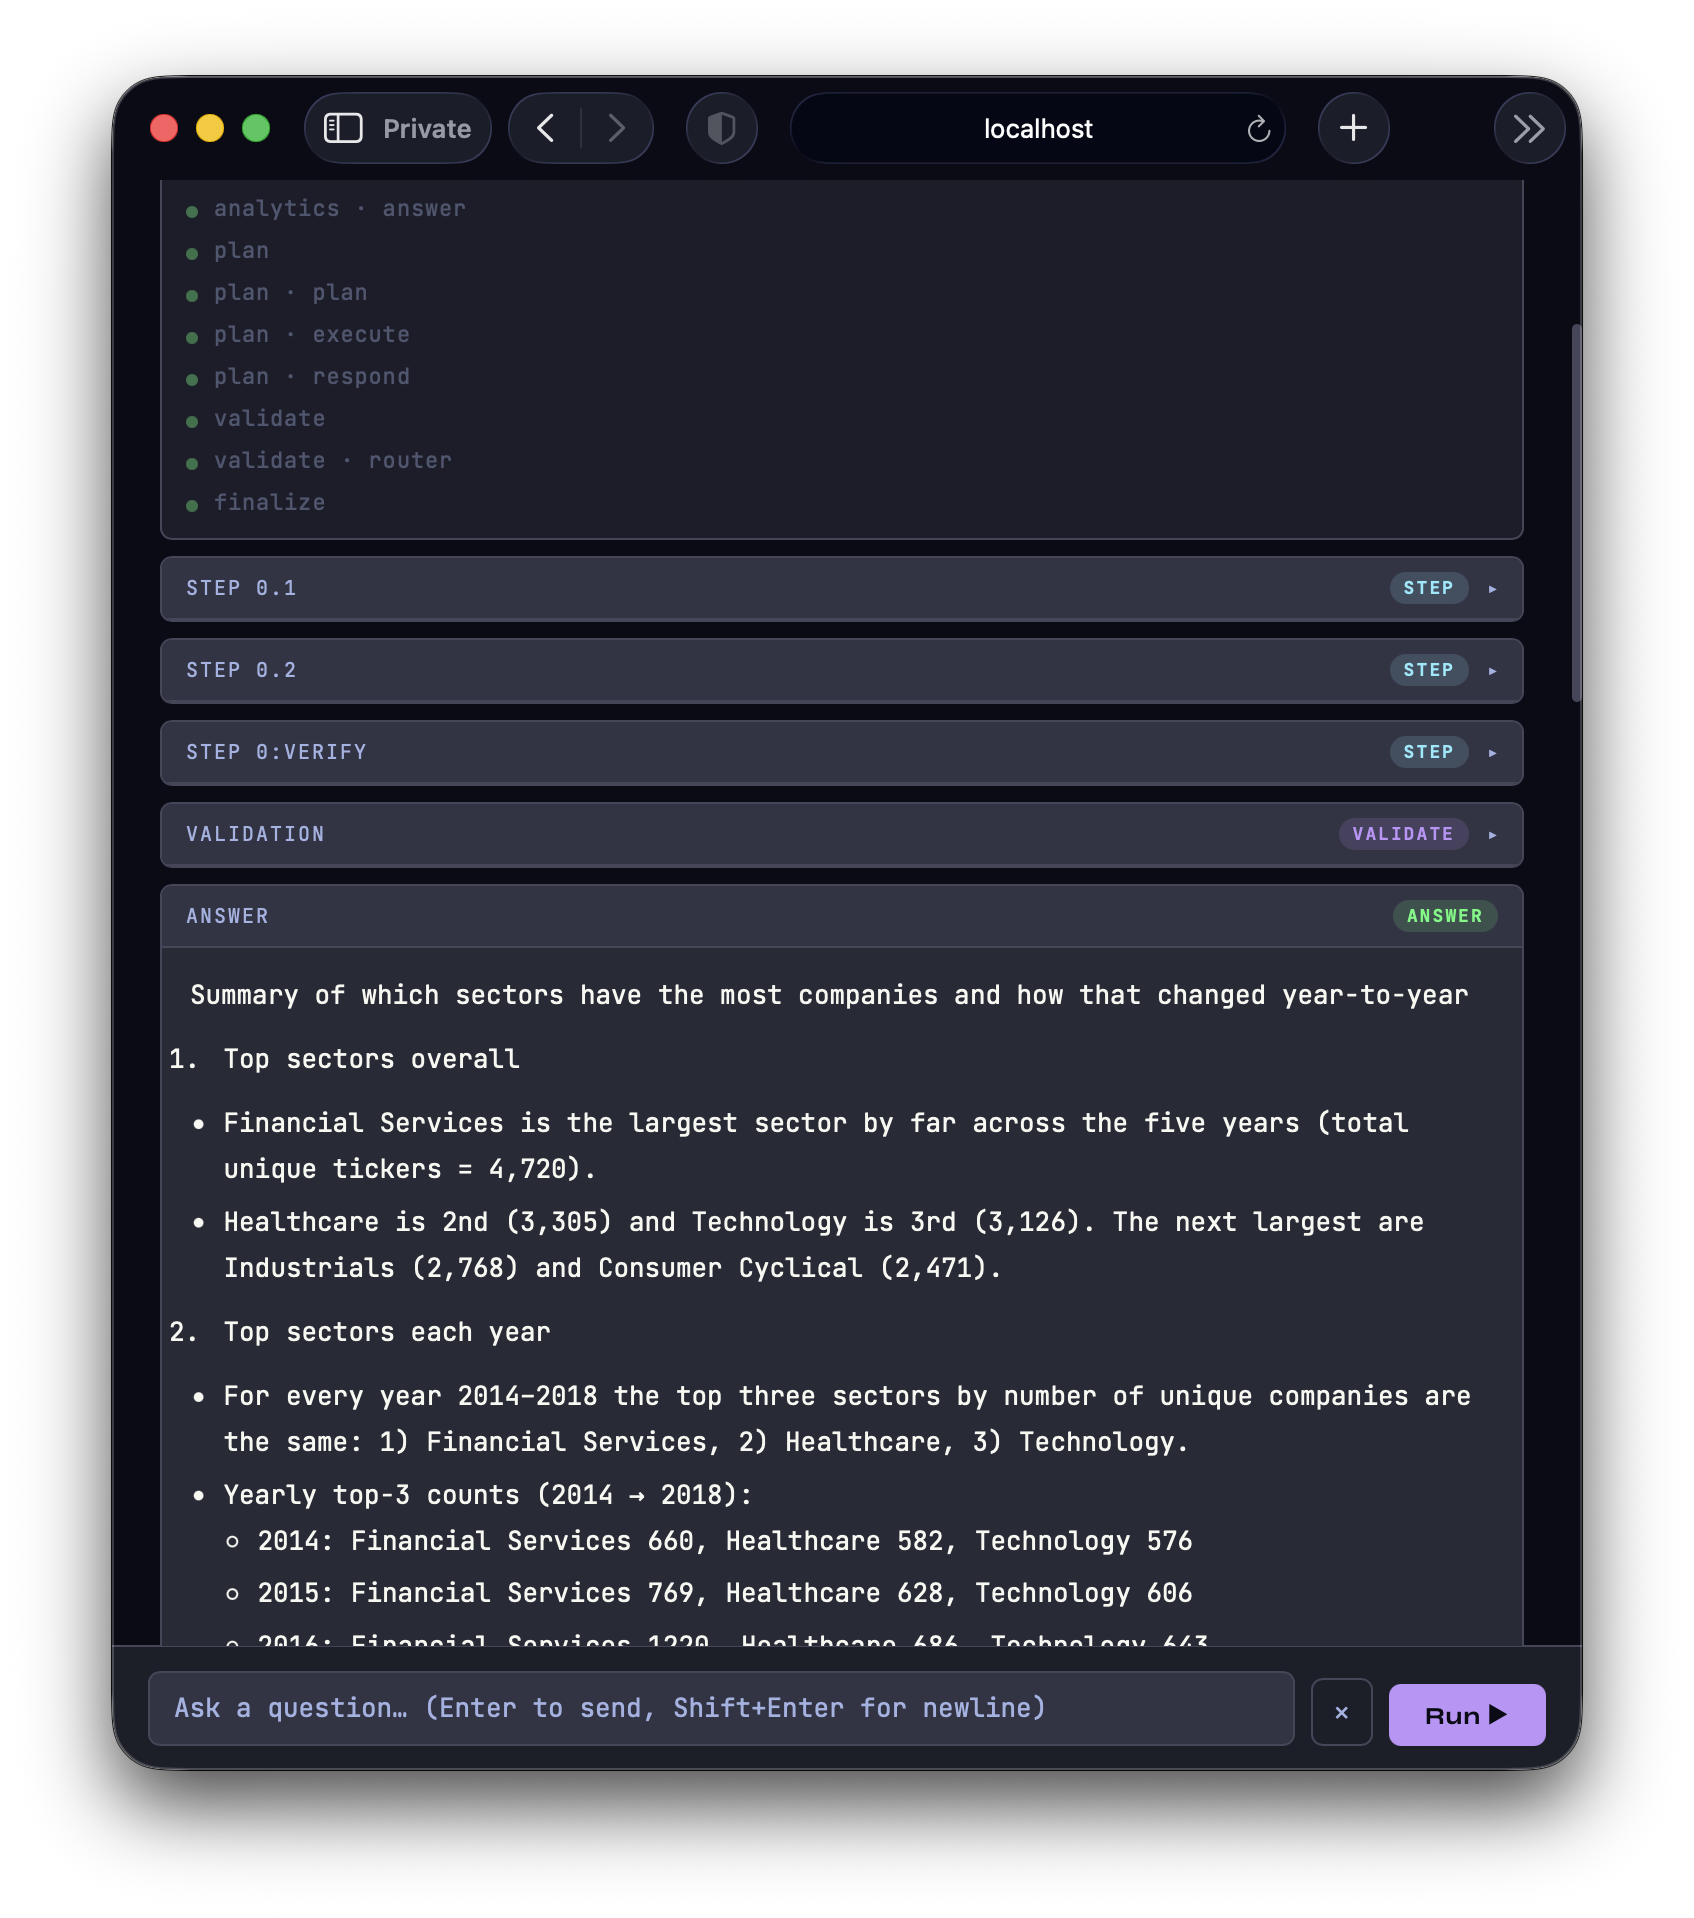
\includegraphics[width=0.4\textwidth]{graphics/ui-which-sectors-have-the-most-companies-represented,-and-how-does-that-distribution-change-year-to-year.png}
  \caption{UI Screenshot}
\end{wrapfigure}

The agent followed a multi-stage analytical workflow. The process combined data aggregation, normalization, ranking, visualization, and interpretation steps before producing the final summary.

\subsect{Understanding the Analytical Objective}

The agent first translated the natural-language question into a quantitative task. It identified that the goal was not simply to count records, but to determine how many distinct companies were represented within each sector for every year. Because companies could appear multiple times within a dataset, the agent chose to count unique ticker symbols rather than raw rows.

The agent also recognized that answering the second part of the question required comparing sector distributions across years, which necessitated both absolute counts and normalized percentages.

\subsect{Extracting Year Information and Preparing Annual Statistics}

The agent processed each yearly financial dataset independently. For every file, it extracted the year from the filename and grouped observations by sector.

Within each sector, the agent computed the number of unique ticker symbols using a distinct-count aggregation. This produced a sector-level company count for each year from 2014 through 2018.

This step transformed the raw company-level datasets into a compact representation that captured the number of companies operating within each sector during each year.

\subsect{Combining Yearly Results into a Unified Table}

After computing annual sector counts, the agent merged the results into a single table with:

\begin{itemize}
  \item sectors as rows,
  \item years as columns, and
  \item unique-company counts as values.
\end{itemize}

Missing sector--year combinations were filled with zeros to ensure consistency across all years. The resulting matrix enabled direct comparison of sector representation over time.

The agent also calculated total company counts across all years for each sector and sorted sectors by these totals. This ranking made it easier to identify the most heavily represented sectors overall.

\subsect{Normalizing Counts to Measure Distribution Changes}

The agent recognized that absolute company counts alone would not fully describe how sector representation changed over time. To measure relative representation, it normalized the counts within each year.

Specifically, the agent divided each sector's count by the total number of companies in that year, producing percentage shares. These percentages allowed the agent to compare sector composition across years even when the total number of companies varied between datasets.

This normalization step was essential for identifying whether changes reflected genuine shifts in sector representation rather than differences in dataset size.

\subsect{Generating Visual Summaries}

\begin{wrapfigure}{l}{0pt}
  \centering
  \includegraphics[width=0.4\textwidth]{report-data/which-sectors-have-the-most-companies-represented,-and-how-does-that-distribution-change-year-to-year/plot-sector-distribution-by-year-stacked.png}
  % \caption{UI Screenshot}
\end{wrapfigure}

To support interpretation, the agent created two visualizations.

First, it produced a stacked bar chart showing sector composition for each year. This visualization highlighted how the overall distribution of companies was allocated among sectors and how those allocations evolved over time.

\begin{wrapfigure}{r}{0pt}
  \centering
  \includegraphics[width=0.4\textwidth]{report-data/which-sectors-have-the-most-companies-represented,-and-how-does-that-distribution-change-year-to-year/plot-top-6-sector-trends.png}
  % \caption{UI Screenshot}
\end{wrapfigure}

Second, it generated a line chart tracking the largest sectors across years. By focusing on the most represented sectors, the chart emphasized long-term trends and made year-to-year changes easier to observe.

These visual outputs complemented the numerical tables and provided a clearer view of temporal patterns.

\subsect{Identifying Dominant Sectors and Yearly Leaders}

With the aggregated data available, the agent examined sector rankings both overall and within individual years.

It computed total company counts across the entire period to determine the most represented sectors overall. It also identified the top sectors within each year by sorting annual counts and extracting the leading categories.

This analysis revealed whether sector leadership changed over time and whether any sectors consistently dominated the dataset.

\subsect{Analyzing Temporal Trends}

The agent then compared both counts and percentage shares across years to identify notable trends.

Rather than merely reporting rankings, it examined how sector representation evolved over time. Particular attention was given to sectors exhibiting unusually large increases or decreases, since these changes were most relevant to the question of distributional change.

The agent compared annual percentages, assessed stability versus volatility among sectors, and highlighted sectors whose representation shifted substantially relative to others.

\subsect{Producing the Final Interpretation}

After completing the quantitative analysis, the agent synthesized the results into a concise narrative. The final response summarized:

\begin{itemize}
  \item the sectors with the largest overall representation,
  \item the leading sectors in each year,
  \item changes in sector shares over time,
  \item notable increases and decreases in representation, and
  \item the broader trends revealed by the visualizations.
\end{itemize}

The final answer therefore emerged from a sequence of reasoning stages: data preparation, unique-company aggregation, cross-year integration, normalization, visualization, ranking, trend analysis, and narrative interpretation.


\break

%
\sect{Analytics Question 2}
%

\begin{wrapfigure}{r}{0pt}
  \centering
  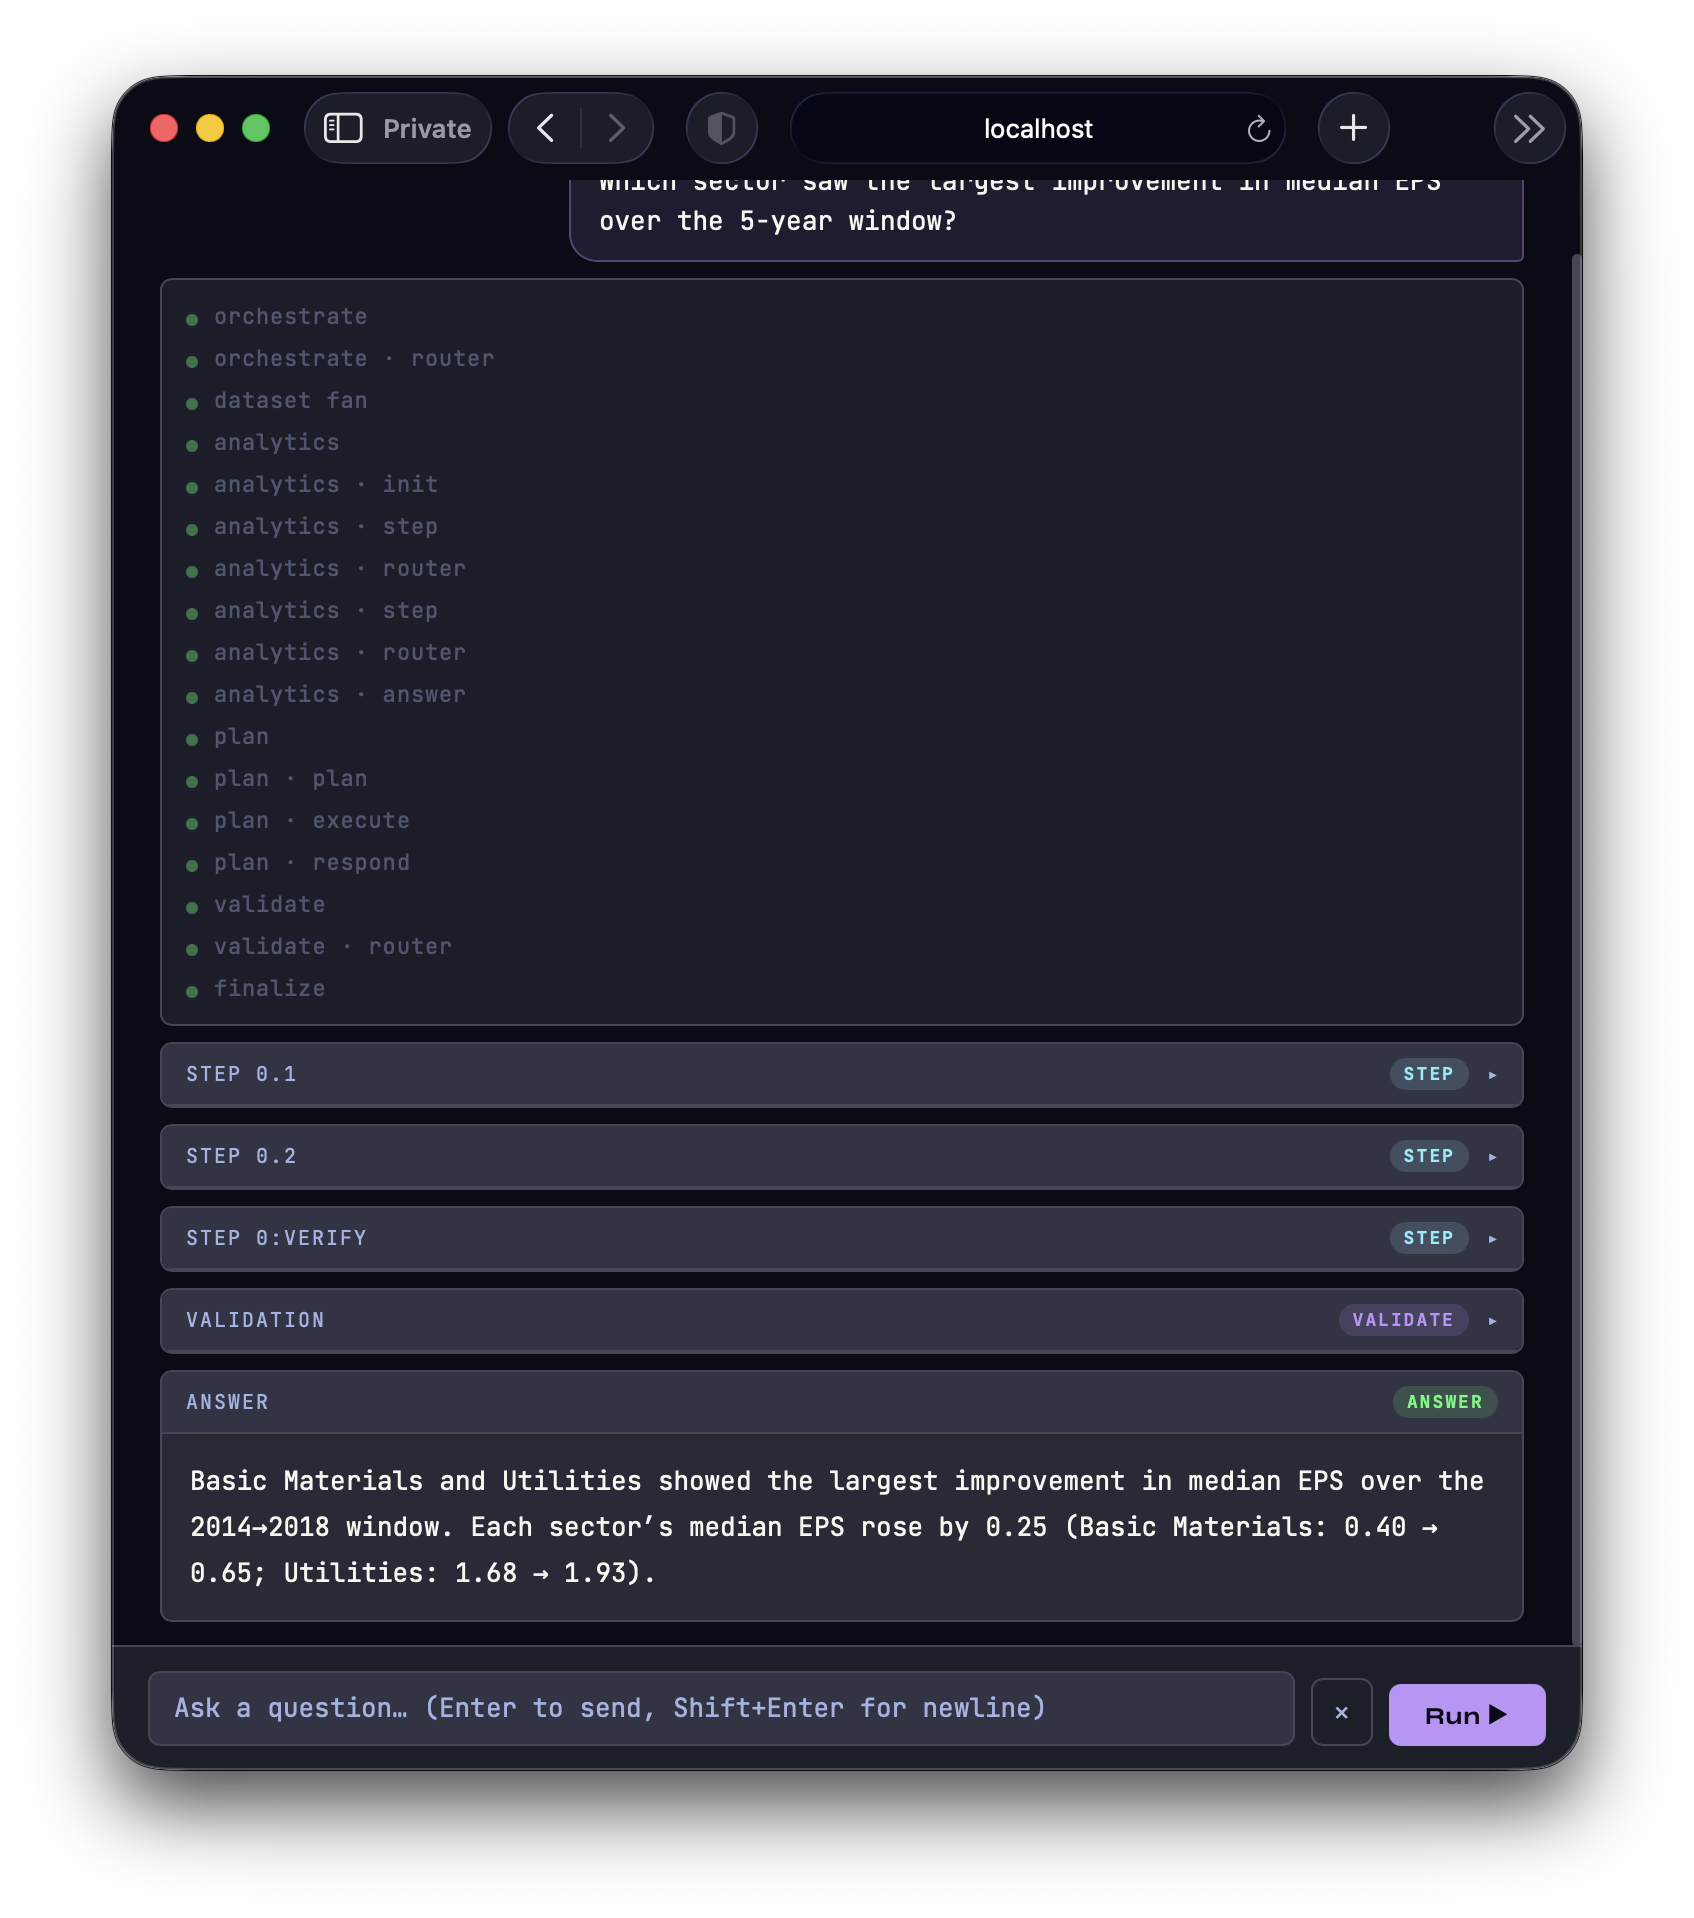
\includegraphics[width=0.4\textwidth]{graphics/ui-which-sector-saw-the-largest-improvement-in-median-eps-over-the-5-year-window.png}
  \caption{UI Screenshot}
\end{wrapfigure}

The agent answers the question by comparing sector-level median earnings per share (EPS) between the beginning and end of the five-year period. Rather than analyzing every intermediate year, it focuses on the net change from 2014 to 2018 and systematically computes the sector-level improvement.

\subsect{Understanding the Analytical Objective}

The agent first interprets the task as a comparison problem. It identifies that the required metric is the change in median EPS for each sector over the five-year window. To answer the question, it plans to:

\begin{itemize}
  \item Compute the median EPS for every sector in 2014.
  \item Compute the median EPS for every sector in 2018.
  \item Compare the two medians by sector.
  \item Identify the sector or sectors with the largest positive change.
\end{itemize}

The agent explicitly defines the improvement metric as:

\[
  \text{Improvement} = \text{Median EPS}_{2018} - \text{Median EPS}_{2014}.
\]

\subsect{Loading and Aggregating the Yearly Data}

Next, the agent loads the financial datasets corresponding to 2014 and 2018. For each dataset, it groups observations by the \texttt{Sector} field and computes the median value of \texttt{EPS}.

This aggregation step transforms thousands of company-level observations into a compact sector-level summary. The resulting outputs are two tables:

\begin{itemize}
  \item Sector median EPS in 2014.
  \item Sector median EPS in 2018.
\end{itemize}

Using medians reduces the influence of extreme EPS values and provides a robust measure of sector performance.

\subsect{Aligning Sector Summaries and Computing Changes}

After obtaining the sector medians for both years, the agent aligns the two summaries by sector and constructs a combined table containing:

\begin{itemize}
  \item Median EPS in 2014.
  \item Median EPS in 2018.
  \item The difference between the two values.
\end{itemize}

The agent also accounts for the possibility that a sector may be missing from one of the years. Any sector lacking a valid median in either year is excluded from the comparison so that the computed change remains meaningful.

\subsect{Identifying the Maximum Improvement}

With the differences calculated, the agent searches for the largest value of the improvement metric. It sorts or scans the sector-level differences and determines the maximum observed increase.

The computed changes reveal that:

\begin{itemize}
  \item Basic Materials improved from 0.40 to 0.65.
  \item Utilities improved from 1.68 to 1.93.
\end{itemize}

Both sectors experienced an increase of:

\[
  0.25 = \text{Median EPS}_{2018} - \text{Median EPS}_{2014}.
\]

\subsect{Handling Ties and Producing the Final Result}

The agent does not assume that only one sector can achieve the maximum improvement. After finding the largest increase, it checks whether multiple sectors share the same value.

This tie-handling step reveals that two sectors achieve the maximum improvement. The agent therefore returns both sectors rather than arbitrarily selecting one.

The final conclusion is that \textbf{Basic Materials} and \textbf{Utilities} tied for the largest improvement in median EPS between 2014 and 2018, with each sector increasing by \textbf{0.25}.

\break

%
\sect{Validator Retry Question 1}
%

\begin{wrapfigure}{l}{0pt}
  \centering
  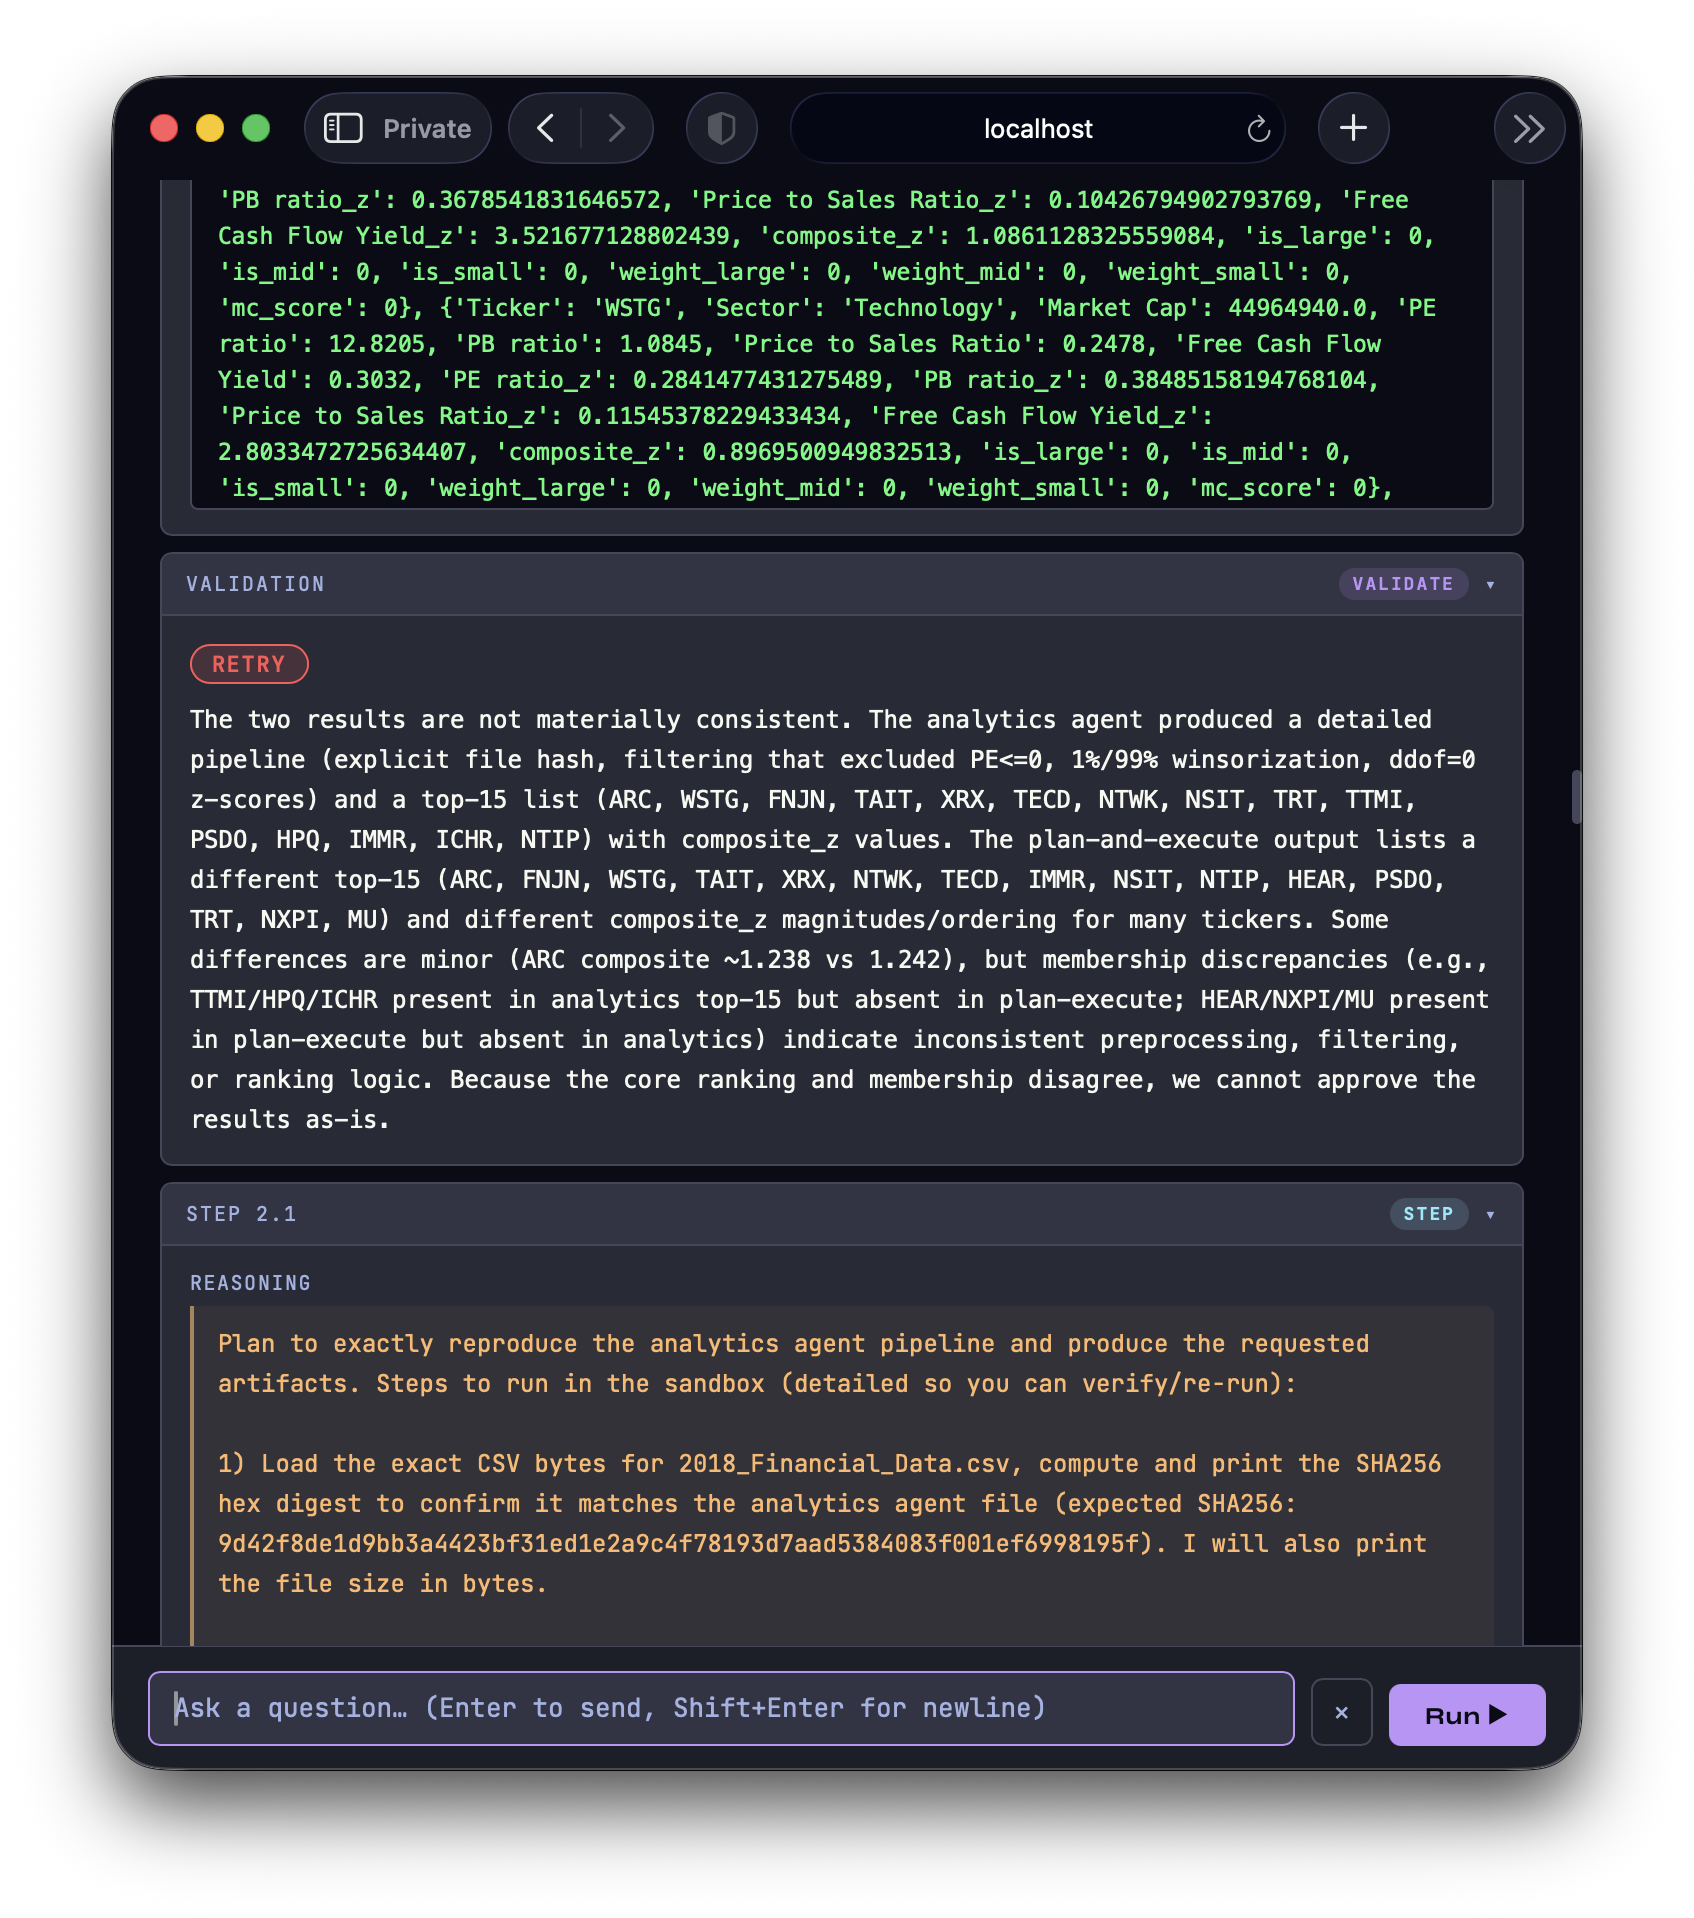
\includegraphics[width=0.4\textwidth]{graphics/ui-find-undervalued-technology-companies-from-the-dataset-produce-plots.png}
  \caption{UI Screenshot}
\end{wrapfigure}

This example demonstrates how the validator agent independently checks the analytics results, identifies inconsistencies, and requests additional analysis before allowing the workflow to continue. The example highlights the purpose of the validator as an independent reasoning component rather than a simple execution checker.

\subsect{Initial Analytics Analysis}

The analytics agent first analyzed the 2018 financial dataset to identify potentially undervalued technology companies. It:

\begin{enumerate}
  \item Loaded the 2018 dataset and filtered companies in the Technology sector.
  \item Selected valuation metrics including PE ratio, PB ratio, Price-to-Sales ratio, and Free Cash Flow Yield.
  \item Cleaned missing values and computed a composite undervaluation score.
  \item Ranked technology companies by this score.
  \item Generated supporting visualizations including scatter plots, bar charts, box plots, and correlation heatmaps.
\end{enumerate}

The analytics agent produced a top-ranked list of undervalued companies and considered the task complete.

\subsect{Validator Detects Inconsistencies}

The validator agent independently reviewed the analytics outputs and compared them against an alternative execution path. During validation, it observed that the rankings generated by different analysis runs were materially different.

The validator noted:

\begin{itemize}
  \item Different top-15 company lists.
  \item Different composite scores for the same companies.
  \item Missing agreement on preprocessing decisions.
  \item Potential inconsistencies in filtering, winsorization, and z-score calculations.
\end{itemize}

The validator therefore issued a \texttt{retry} verdict rather than approving the result. Specifically, it identified disagreements such as:

\begin{itemize}
  \item Different companies appearing in the top-ranked results.
  \item Different ranking orders.
  \item Different composite score magnitudes.
\end{itemize}

Because the numerical outputs could not be independently verified, the validator concluded that the analysis was not yet trustworthy.

\subsect{Validator Feedback Request}

Instead of simply rejecting the result, the validator generated a detailed remediation plan. It requested that the analytics workflow be rerun using a fully specified canonical pipeline.

The validator required the following information:

\begin{enumerate}
  \item Confirmation of the exact input dataset and SHA256 hash.
  \item Explicit Technology-sector filtering rules.
  \item Treatment of PE values less than or equal to zero.
  \item Counts before and after each filtering step.
  \item Exact winsorization boundaries.
  \item Exact z-score computation parameters.
  \item Directionality of each valuation metric.
  \item A reproducible top-30 output table.
  \item Source code used for the computation.
  \item Regeneration of all supporting plots.
\end{enumerate}

This feedback demonstrates that the validator reasons about correctness and reproducibility rather than merely checking whether code executed successfully.

\subsect{Retry Execution}

After receiving validator feedback, the analytics workflow was executed again with a stricter and fully documented pipeline.

The retry execution performed the following steps:

\begin{enumerate}
  \item Verified the dataset being used.
  \item Applied an exact case-insensitive filter:
    \texttt{Sector == "technology"}.
  \item Treated all PE values $\leq 0$ as missing.
  \item Dropped rows missing any required valuation metric.
  \item Applied 1\%/99\% winsorization.
  \item Computed z-scores using population standard deviation (\texttt{ddof=0}).
  \item Inverted PE, PB, and Price-to-Sales z-scores.
  \item Kept Free Cash Flow Yield positive.
  \item Computed the composite score as the average of the directional z-scores.
  \item Generated a reproducible top-30 CSV, plots, and processing script.
\end{enumerate}

The retry run also reported intermediate diagnostics such as:

\begin{itemize}
  \item Total rows: 4392
  \item Technology rows: 636
  \item Final rows after cleaning: 293
  \item Winsorization thresholds for all four metrics
  \item Means and standard deviations used in z-score calculations
\end{itemize}

\subsect{Validator Re-Validation}

Following the retry execution, the validator compared the newly generated outputs against the requested canonical specification.

The validator verified:

\begin{itemize}
  \item Matching row counts after preprocessing.
  \item Matching winsorization thresholds.
  \item Consistent z-score computation parameters.
  \item Correct handling of PE values.
  \item Availability of reproducible CSV outputs and scripts.
\end{itemize}

The retry process resolved the ambiguity that existed in the earlier analysis and produced a reproducible workflow suitable for validation.

\subsect{Key Observation}

This example illustrates the primary role of the validator agent in the HW4 architecture. The validator does not merely inspect execution success; it independently reasons about numerical correctness, reproducibility, preprocessing consistency, and completeness of analysis. When discrepancies are detected, the validator generates concrete corrective actions and forces an additional reasoning/execution cycle before the system can proceed.


\break

%
\sect{Validator Retry Question 2}
%

\begin{wrapfigure}{r}{0pt}
  \centering
  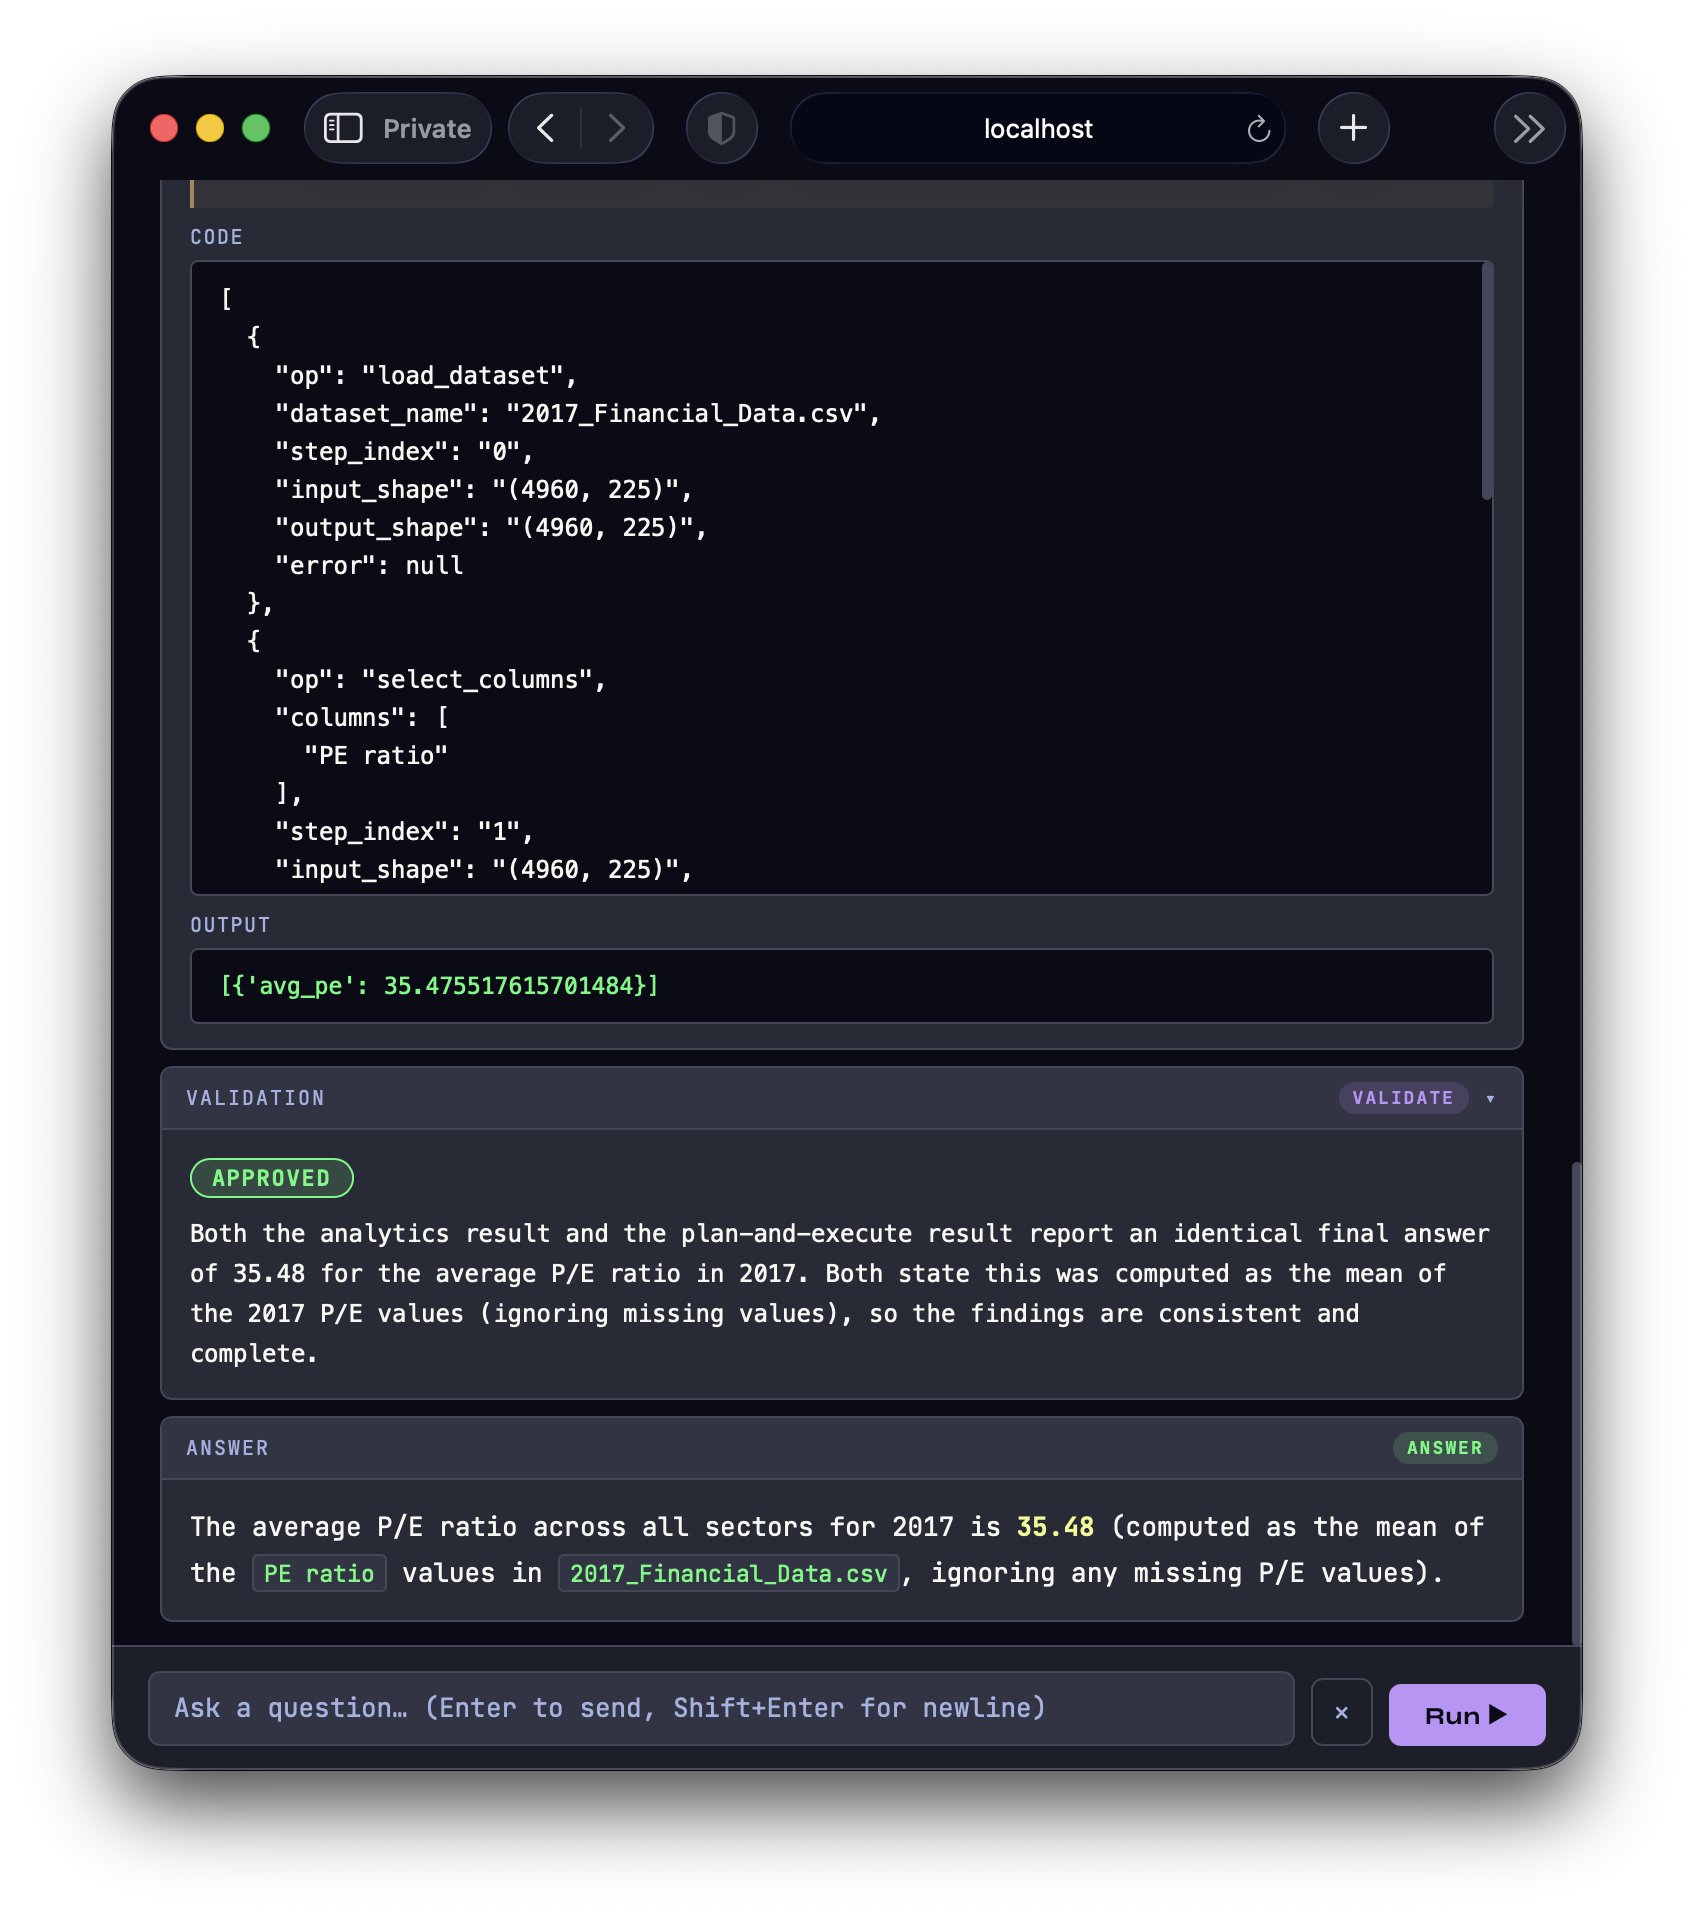
\includegraphics[width=0.4\textwidth]{graphics/ui-what-is-the-average-p-e-ratio-across-all-sectors-for-2017.png}
  \caption{UI Screenshot}
\end{wrapfigure}

This example demonstrates a successful execution in which the validator approves the result on the first attempt. No retry requests are issued because the independent solution paths agree on the final answer.

From the input specification, it identifies a single dataset, \texttt{2017\_Financial\_Data.csv}. The task is interpreted as computing the overall mean of the \texttt{PE ratio} column across all rows in the dataset. The agent explicitly notes that missing values should be ignored when computing the mean.

\subsect{Analytics Agent Execution}

The analytics agent performs a direct computation using Python. It:

\begin{enumerate}
  \item Loads \texttt{2017\_Financial\_Data.csv}.
  \item Converts the \texttt{PE ratio} column to numeric values.
  \item Computes the mean using \texttt{mean(skipna=True)}.
  \item Produces the result:
    \[
      35.475517615701484
    \]
\end{enumerate}

The agent then rounds the value for presentation and generates the answer:

\begin{quote}
  The average P/E ratio across all sectors for 2017 is \textbf{35.48}.
\end{quote}

A follow-up analytics reasoning step verifies that no additional computation is required because the requested quantity is a single global average.

\subsect{Plan-and-Execute Agent}

In parallel, the planning agent constructs an explicit execution plan. The plan consists of four operations:

\begin{enumerate}
  \item \texttt{load\_dataset} on \texttt{2017\_Financial\_Data.csv}.
  \item \texttt{select\_columns} to retain only \texttt{PE ratio}.
  \item \texttt{group\_aggregate} with an empty grouping key, computing the mean of \texttt{PE ratio}.
  \item \texttt{display} the resulting single-row output.
\end{enumerate}

The planner therefore reaches the same numerical result and produces the answer:

\begin{quote}
  The average P/E ratio across all sectors for 2017 is 35.48.
\end{quote}

\subsect{Validation Agent}

The validation agent compares the outputs of the analytics pipeline and the plan-and-execute pipeline.

It verifies that:

\begin{itemize}
  \item Both methods compute the mean of the 2017 \texttt{PE ratio} values.
  \item Both explicitly ignore missing values.
  \item Both produce the identical final answer, \(35.48\).
\end{itemize}

The validator records the verdict:

\begin{quote}
  \texttt{approved}
\end{quote}

The validator's reasoning states that the findings are consistent and complete because the independently generated solutions agree exactly.

\subsect{Retry Analysis}

No retry cycle occurs in this example.

The validation output contains:

\begin{itemize}
  \item Verdict: \texttt{approved}
  \item Feedback: \texttt{null}
\end{itemize}

Because no discrepancies, execution errors, or inconsistencies are detected, the validator does not request additional work from either agent. The workflow therefore terminates after the initial validation pass.

\subsect{Final Outcome}

The system successfully answers the question on the first attempt. Agreement between the analytics agent and the plan-and-execute agent allows the validator to approve the result immediately, eliminating the need for any retry requests or corrective actions.


\break

%
%
\chap{End-to-End Analytics Scenario}
%
%

\input{report-sections/06-scenario}

%
%
\chap{Iterative Reasoning Deep Dives}
%
%

%
\sect{Deep Dive A}
%

\input{report-sections/07-deep-dive-a}

%
\sect{Deep Dive B}
%

\input{report-sections/07-deep-dive-b}

%
%
\chap{Presentation Summary}
%
%

\input{report-sections/08-presentation-summary}

%
%
\chap{Discussion}
%
%

%
\sect{Limitations}
%

\input{report-sections/09-limitations}

%
\sect{Lessons Learned}
%

\input{report-sections/09-lessons-learned}

%
\sect{Future Work}
%

\input{report-sections/09-future-work}

%
%
\chap{Conclusion}
%
%

\input{report-sections/10-conclusion}

\end{document}
